\begin{frame}{2.1 Arsitektur Sirkuit QPhE (3-bit Phase)}
    \begin{columns}
        \begin{column}{0.6\textwidth}
            \centering
            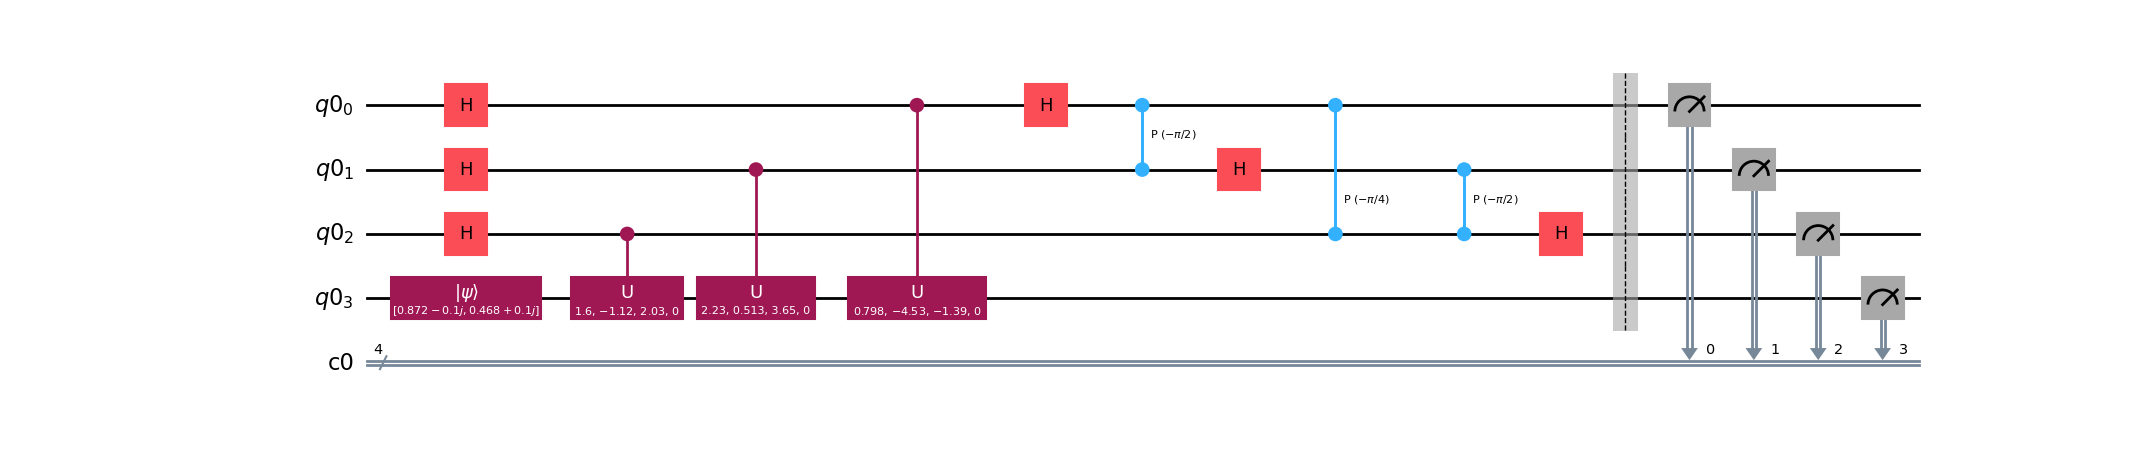
\includegraphics[width=\textwidth]{../QPCA-master/circuit_qphe.png}
            \captionof{figure}{Sirkuit QPhE dengan 3-qubit Register Fase}
        \end{column}
        \begin{column}{0.4\textwidth}
            \small
            \begin{itemize}
                \item \textbf{Register Fase ($q_0-q_2$):} Menggunakan 3 qubit untuk resolusi spektral $2^3 = 8$ level.
                \item \textbf{Register Target ($q_3$):} Menyandikan \textit{eigenvector} volatilitas awal.
                \item \textbf{Mekanisme CU:} Pemetaan nilai spektral ke dalam fase register melalui gerbang terkontrol.
            \end{itemize}
        \end{column}
    \end{columns}
\end{frame}

\begin{frame}{2.2 Dekomposisi Sirkuit: Transpiled QPhE}
    \begin{columns}
        \begin{column}{0.6\textwidth}
            \centering
            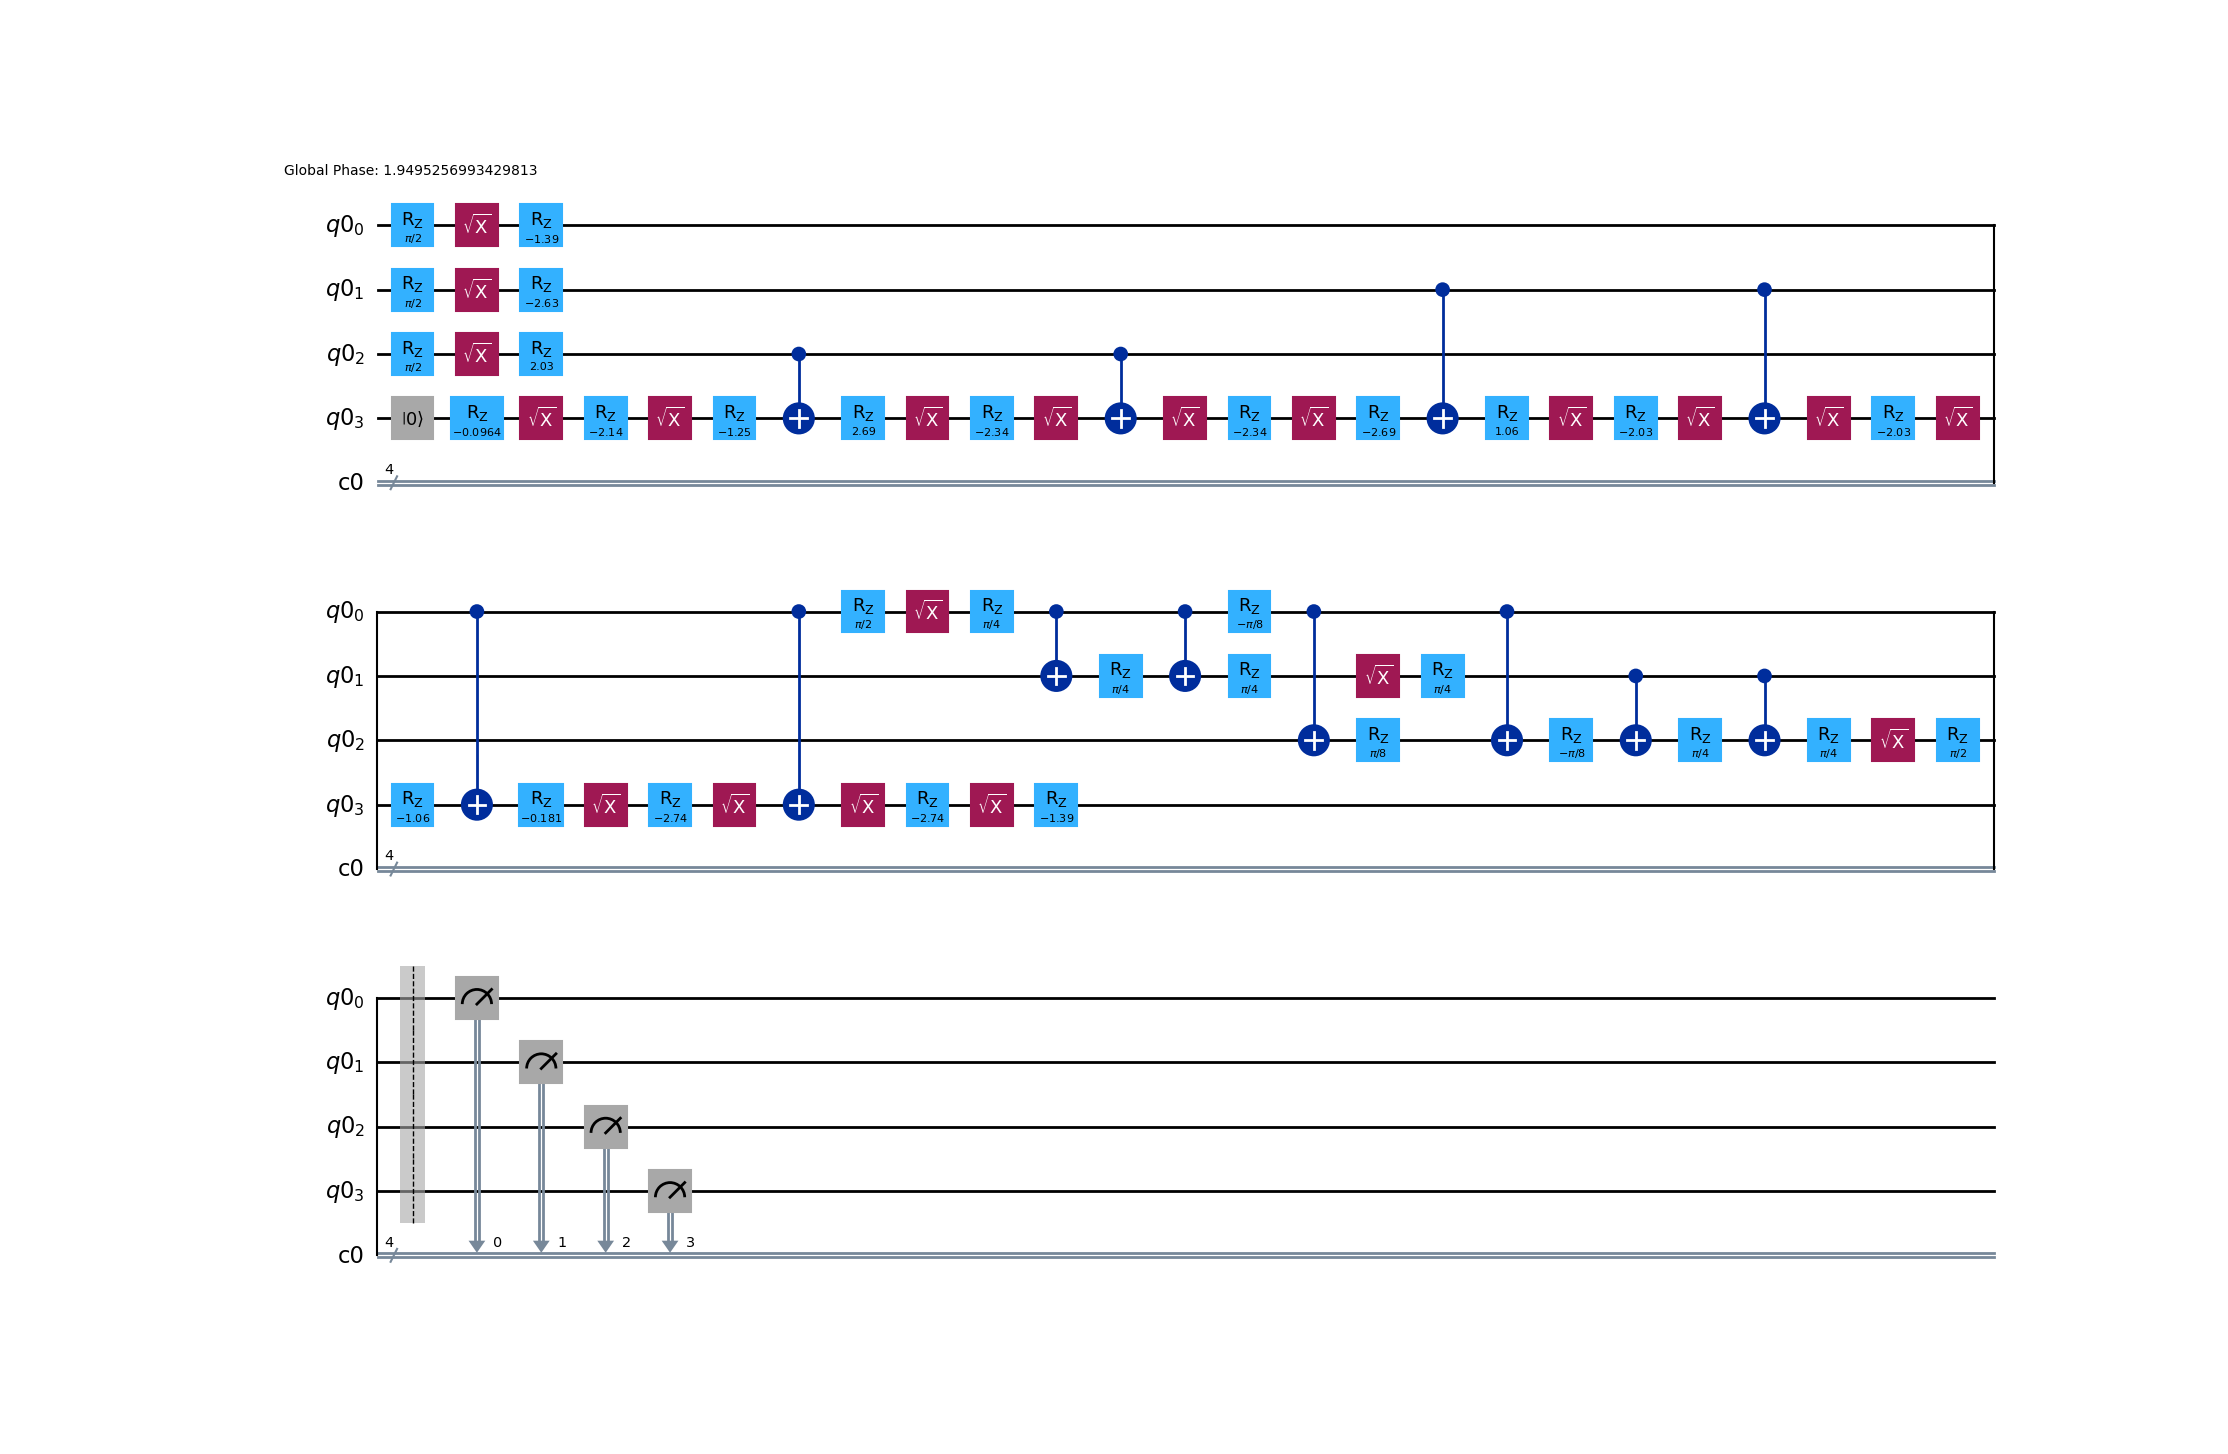
\includegraphics[width=\textwidth]{../QPCA-master/circuit_transpiled_qphe.png}
            \captionof{figure}{Sirkuit QPhE setelah Transpilasi}
        \end{column}
        \begin{column}{0.4\textwidth}
            \small
            \begin{itemize}
                \item \textbf{Basis Gates:} Gerbang $CU$ tingkat tinggi didekomposisi menjadi gerbang fisik $U3$ dan $CX$.
                \item \textbf{Kedalaman Logis:} Transpilasi mengungkap jumlah gerbang CNOT yang sebenarnya, yang menjadi sumber utama derau pada perangkat NISQ.
                \item \textbf{Optimasi:} Struktur ini menunjukkan bagaimana Qiskit memetakan algoritma ke topologi qubit IBMQX2.
            \end{itemize}
        \end{column}
    \end{columns}
\end{frame}

\begin{frame}{2.3 Distribusi Spektral dan Estimasi Utama}
    \begin{columns}
        \begin{column}{0.5\textwidth}
            \begin{itemize}
                \item \textbf{Analisis Histogram:} Puncak dominan pada bitstring \textit{0000} dan \textit{1000} menunjukkan konvergensi register fase ($c_2c_1c_0$) pada state $|000\rangle$.
                \item \textbf{Interpretasi Eigenvalue:} Hasil $y=0$ memberikan estimasi $\Lambda = 1.0$, merepresentasikan komponen volatilitas utama.
                \item \textbf{Dualitas Target:} Keberadaan dua bar tinggi mengonfirmasi bahwa \textit{eigenvector} berada dalam superposisi $|0\rangle$ dan $|1\rangle$.
            \end{itemize}
        \end{column}
        \begin{column}{0.5\textwidth}
            \centering
            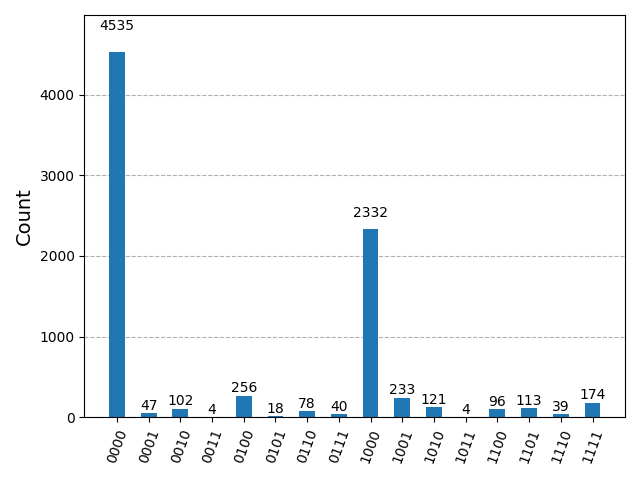
\includegraphics[width=\textwidth]{../QPCA-master/qpca_qphe_result.png}
            \captionof{figure}{Estimasi Eigenvalue Utama}
        \end{column}
    \end{columns}
\end{frame}

\begin{frame}{2.4 Tomografi State: Analisis Struktur State City}
    \begin{columns}
        \begin{column}{0.5\textwidth}
            \centering
            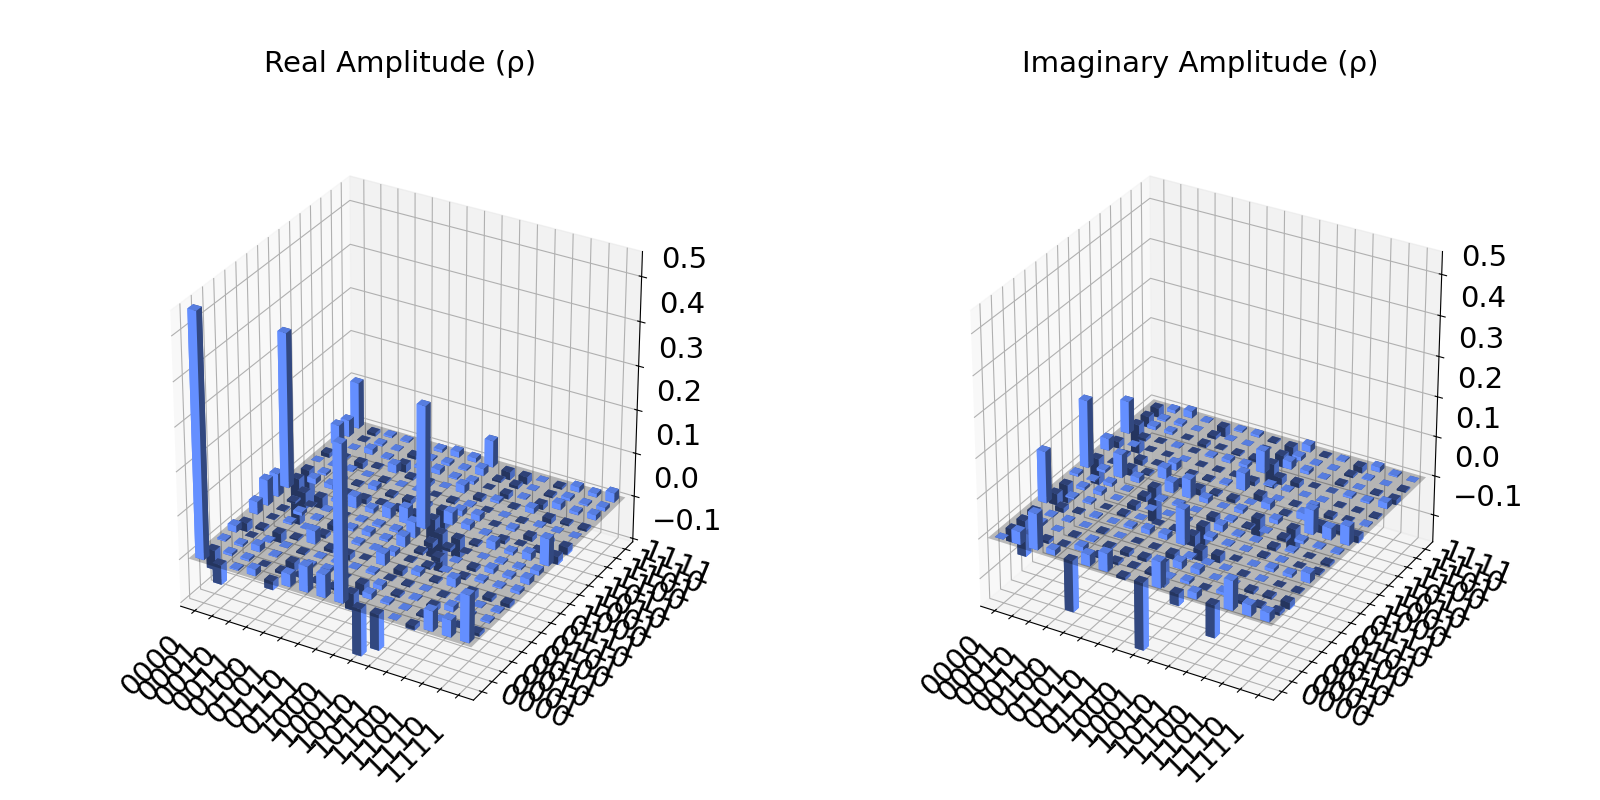
\includegraphics[width=\textwidth]{../QPCA-master/state_city_qphe.png}
            \captionof{figure}{Matriks Densitas (Elemen Riil)}
        \end{column}
        \begin{column}{0.5\textwidth}
            \small
            \begin{itemize}
                \item \textbf{Karakteristik Bar:} Dalam gambar ditunjukkan bahwa indeks basis \textit{(0000, 0000)} menunjukkan bar positif, sedangkan \textit{(1000, 1000)} menunjukkan bar negatif secara fase.
                \item \textbf{Makna Fisik:} Perbedaan fase pada elemen diagonal merepresentasikan koherensi internal \textit{eigenvector} yang diekstraksi.
            \end{itemize}
        \end{column}
    \end{columns}
\end{frame}

\begin{frame}{2.5 Korelasi Antar Register pada Hinton Map}
    \begin{columns}
        \begin{column}{0.5\textwidth}
            \centering
            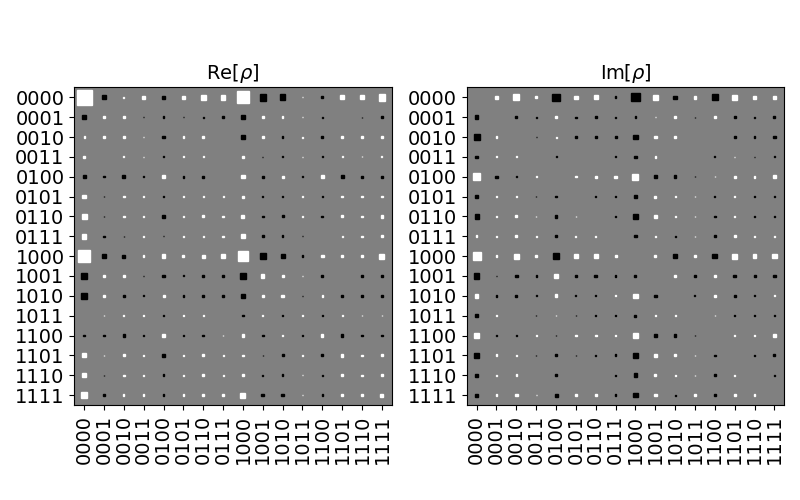
\includegraphics[width=0.9\textwidth]{../QPCA-master/hinton_qphe.png}
            \captionof{figure}{Peta Distribusi Amplitudo Hinton}
        \end{column}
        \begin{column}{0.5\textwidth}
            \small
            \begin{itemize}
                \item \textbf{Ukuran Kotak:} Luas area kotak putih pada koordinat $|000\rangle$ menunjukkan probabilitas dominan untuk eigenvalue tersebut.
                \item \textbf{Entanglement:} Kotak yang terdefinisi jelas pada kolom fase yang bersilangan dengan baris target menunjukkan keberhasilan pemetaan spektral.
            \end{itemize}
        \end{column}
    \end{columns}
\end{frame}

\begin{frame}{2.6 Orientasi Geometris pada Multivektor Bloch}
    \begin{columns}
        \begin{column}{0.5\textwidth}
            \centering
            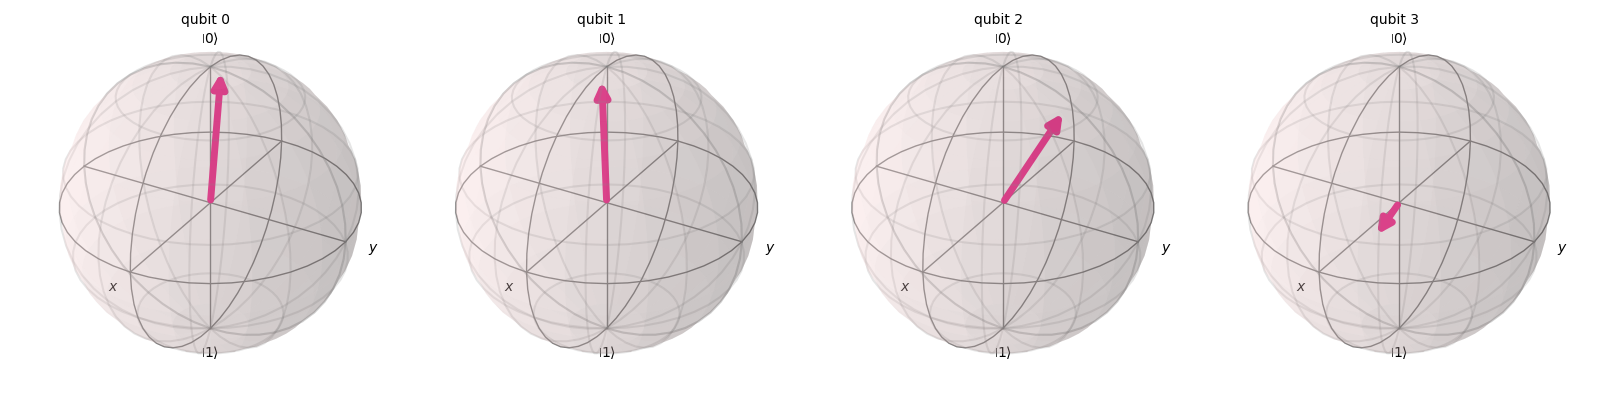
\includegraphics[width=\textwidth]{../QPCA-master/bloch_qphe.png}
            \captionof{figure}{Posisi Vektor pada Bola Bloch}
        \end{column}
        \begin{column}{0.5\textwidth}
            \small
            \begin{itemize}
                \item \textbf{Visualisasi Vektor:} Vektor $q_0-q_2$ dan $q_3$ berada pada posisi \textbf{statis} di permukaan bola antara sumbu $|0\rangle$, $+x$, dan $+y$.
                \item \textbf{Fungsionalitas:} Register fase diarahkan untuk estimasi biner, sementara $q_3$ menyandikan data kontinu \textit{eigenvector}.
                \item \textbf{Integritas:} Panjang vektor $r \approx 1$ mengonfirmasi kemurnian informasi tanpa gangguan dekoherensi signifikan.
            \end{itemize}
        \end{column}
    \end{columns}
\end{frame}
